\documentclass[12pt,a4paper]{article}

% --- Packages ---
\usepackage[utf8]{inputenc}
\usepackage[T1]{fontenc}

\usepackage{amsmath,amssymb,amsfonts,amsthm}
\usepackage{graphicx}
\usepackage{multirow}
\usepackage{algorithmic}
\usepackage{textcomp}
\usepackage{xcolor}
\usepackage{cite}
\usepackage{url}
\usepackage{listings}
\usepackage{xcolor}
\usepackage{float}


\lstset{
    language=Python,
    basicstyle=\ttfamily\small,
    numbers=left,
    numberstyle=\tiny\color{gray},
    frame=single,
    breaklines=true,
    showstringspaces=false,
    keepspaces=true
}

% --- Page Layout ---
\usepackage{geometry}
\geometry{margin=1in}

% --- Hyperlinks ---
\usepackage{hyperref}
\hypersetup{
    hidelinks,
    colorlinks=false
}

% --- Document Info ---
\title{\small{MATH 425}\\\huge{Individual Assignment : Queue Simulation}}
\author{
    Ndeye Anta MBAYE
}
\date{\today}

\begin{document}

\maketitle


% --- Main Content ---
\section{Python Code for Queue Simulation}
\begin{lstlisting}
# Author: Ndeye Anta Mbaye
# Date: 19 September 2026
# simulation.py

# Imports
import numpy as np
import pandas as pd
import matplotlib.pyplot as plt

# Simulate 1,000 scenarios.
scenarios = []

# For each scenario:
for i in range(1000):
    # Generate the arrival rate, lambda, randomly between 8 and 12 customers/hour.
    arrival_rate = np.random.uniform(low=8, high=12)
    # Generate the current service rate, mu, randomly between 13 and 17 customers/hour.
    service_rate = np.random.uniform(low=13, high=17)

    # For each scenario, calculate rho, Ls, Lq, Ws, Wq
    rho = arrival_rate / service_rate
    ls = rho / (1-rho)
    lq = ls-rho
    ws=ls/arrival_rate
    wq=lq/arrival_rate

    # Append the scenarios to the array
    scenarios.append({
        'arrival_rate': arrival_rate,
        'service_rate': service_rate,
        'rho': rho,
        'ls': ls,
        'lq': lq,
        'ws': ws,
        'wq': wq
    })

# Create histograms showing the distributions of rho, Ls, Lq, Ws, and Wq
keys = ["rho", "ls", "lq", "ws", "wq"]
for key in keys:
    values = [scenario[key] for scenario in scenarios]
    plt.hist(values, bins=30)
    plt.title(f"Distribution of {key} with 30 bins")
    plt.xlabel(key)
    plt.ylabel("Frequency")
    plt.show()

# Save the simulation results as a CSV file
pd.DataFrame(scenarios).to_csv("results/scenarios.csv", index=False)

# Find the descriptive stats
stats = []
labels = ["arrival_rate", "service_rate", "rho", "ls", "lq", "ws", "wq"]

for label in labels:
    values = [scenario[label] for scenario in scenarios]

    # Find the stats for each metric and append to array
    stats.append({
        "variable": label,
        "mean": round(np.mean(values),3),
        "median": round(np.median(values),3),
        "mode": pd.Series(values).mode().iloc[0],
        "standard deviation": np.std(values),
        "min": np.min(values),
        "max": np.max(values)
    })

# Save descriptive statistics as csv
pd.DataFrame(stats).round(3).to_csv("results/descriptive_statistics.csv", index=False)


# Assume management wants at least 95% of customers to wait no more than 15 minutes.
# Use the M/M/1 relationship, P(Wq > t) = rho * exp[-(mu-lambda)t]  where t = 15/60 hours.
results = []
percentiles = [50, 75, 90, 95, 97.5]

# Use the 97.5th percentile of lambda as the design demand level.
# Repeat the capacity calculation using the 50th, 75th, 90th, 95th, and 97.5th percentiles of demand.
for percentile in percentiles:
    lambda_p = np.percentile([scenario["arrival_rate"] for scenario in scenarios], percentile)
    # Determine the minimum service rate mu required to achieve the 95% target.
    min_rate = lambda_p

    while (lambda_p / min_rate) * np.exp(-(min_rate - lambda_p) * (15 / 60)) > 0.05:
        min_rate += 0.01

    rho = lambda_p / min_rate
    p= rho * np.exp(-(min_rate - lambda_p) * (15 / 60))
    results.append({
        "lambda": lambda_p,
        "min_rate": min_rate,
        "rho": rho,
        "probability": p,
    })

# Sensitivity table
sensitivity_table = pd.DataFrame(results, index=[f"{p}th percentile" for p in percentiles], columns=["lambda", "min_rate", "rho", "probability"])
print(sensitivity_table)
\end{lstlisting}

\section{Histograms}
\begin{figure}[H]
    \centering
    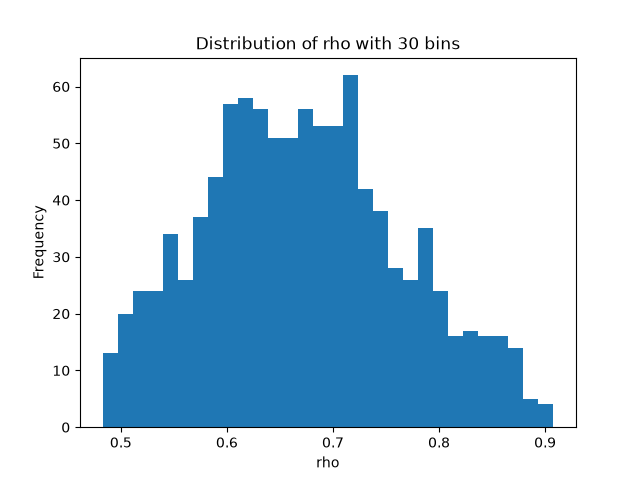
\includegraphics[width=0.8\textwidth]{figures/rho.png}
    \caption{Distribution of $\rho$}
\end{figure}

\begin{figure}[H]
    \centering
    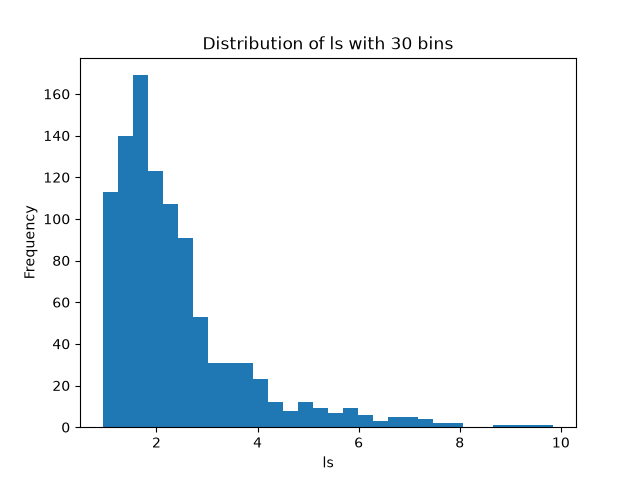
\includegraphics[width=0.8\textwidth]{figures/ls.png}
    \caption{Distribution of Ls}
\end{figure}

\begin{figure}[H]
    \centering
    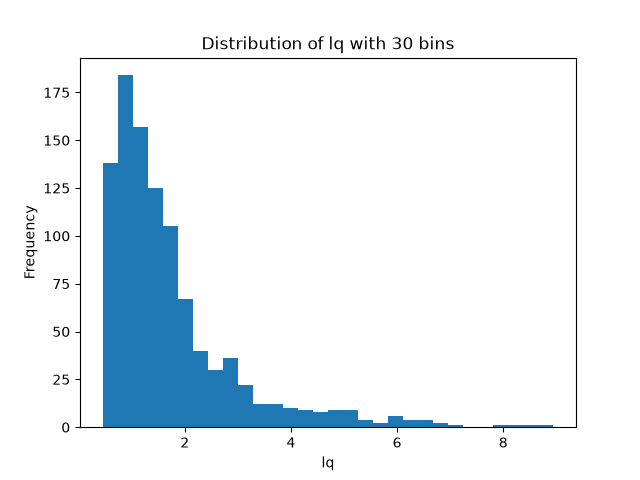
\includegraphics[width=0.8\textwidth]{figures/lq.png}
    \caption{Distribution of Lq}
\end{figure}

\begin{figure}[H]
    \centering
    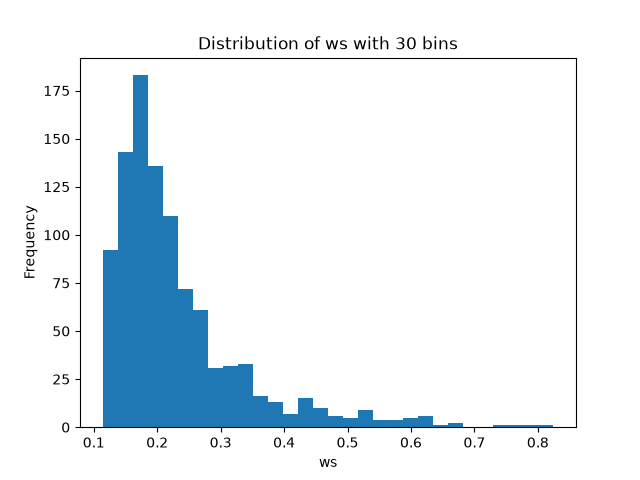
\includegraphics[width=0.8\textwidth]{figures/ws.png}
    \caption{Distributions of Ws}
\end{figure}

\begin{figure}[H]
    \centering
    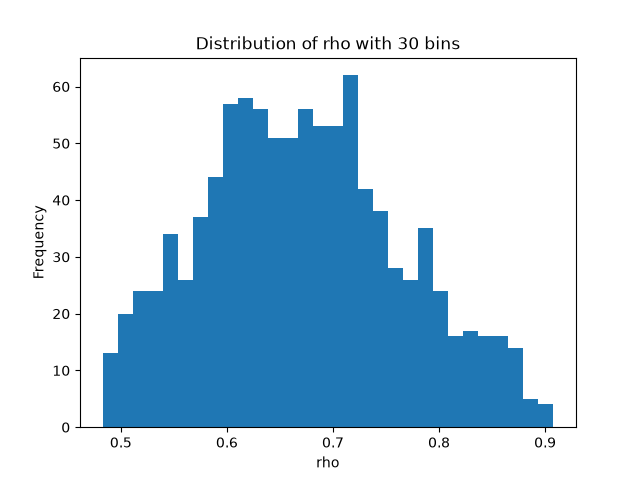
\includegraphics[width=0.8\textwidth]{figures/rho.png}
    \caption{Distributions of Wq}
\end{figure}
\section{Sensitivity Analysis Table}
\begin{figure}[H]
    \centering
    \includegraphics[width=0.8\textwidth]{figures/sensitivity.png}
    \caption{Sensitivity Analysis Table}
\end{figure}
\section{Service Capacity Decision Table}
\begin{figure}[H]
    \centering
    \includegraphics[width=0.8\textwidth]{figures/scd.png}
    \caption{Service Capacity Decision Table}
\end{figure}
\section{Results Interpretation}
The simulation results show that the arrival and service rates vary within their respective ranges,
leading to different values of $\rho$, $L_s$, $L_q$, $W_s$, and $W_q$, which affect the performance of 
the queueing system differently.
The histograms illustrate the distributions of these metrics across the 1,000 simulated scenarios.

The arrival rate for the 97.5th percentile is approximately 11.9 customers/hour, and the minimum service rate required to achieve the 95% target is approximately 21.5 customers/hour.
The sensitivity analysis table shows that the arrival and minimum service rates increase
as we move from the 50th to the 97.5th percentile, indicating that higher demand levels require higher service rates to maintain the desired performance level.
\end{document}